\documentclass{beamer}
\usepackage{tikz}
\usepackage{graphicx}
\usetikzlibrary{arrows.meta}
\tikzset{>={Latex[width=2mm,length=2mm]}}

\begin{document}

\begin{tikzpicture}[scale=1,font=\footnotesize]
\tikzstyle{s}=[circle,draw,inner sep=2,fill=black]
\tikzstyle{h}=[circle,draw, inner sep=2]
    
    \node[s] (1) at (0,0){};
    \node[s, label={[align=center]Excess\\credit}] (2) at (1,2){};
    \node[s, label={[align=center]Financial\\recession}] (3) at (4,2){};
    \node[s] (4) at (4,-2){};
    \node[s] (5) at (6,0){};
    \node[state, label={[align=center]Macrocontrols}] (7) at (-1,0){};
    \node[state, label={[align=center]Output}] (8) at (6.5,-0.1){};
    \node[state, label={[align=center, below]Normal\\recession}] (4) at (4,-2.2){};
    
    \draw[->] (1) edge (2);
    \draw[->] (1) edge (3);
    \draw[->] (1) edge (4);
    \draw[->] (2) edge (5);
    \draw[->] (2) edge (3);
    \draw[->] (2) edge (4);
    \draw[->] (3) edge (5);
    \draw[->] (4) edge (5);
    \draw[->] (1) edge (5);
    
\end{tikzpicture}

\begin{frame}{}
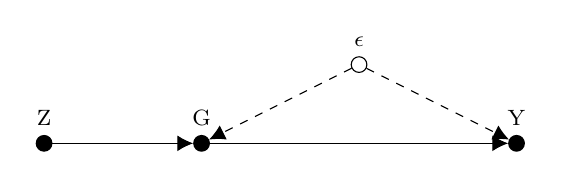
\begin{tikzpicture}[scale=1,font=\footnotesize]
\tikzstyle{s}=[circle,draw,inner sep=2,fill=black]
\tikzstyle{h}=[circle,draw, inner sep=2]
    
    \node[s, label=Z] (1) at (0,0){};
    \node[s, label=G] (2) at (2,0){};
    \node[s, label=Y] (3) at (6,0){};
    \node[h, label=$\epsilon$] (4) at (4,1){};
    
  
    \draw[->] (1) edge (2);
    \draw[->] (2) edge (3);
    \draw[->][dashed] (4) edge (2);
    \draw[->][dashed] (4) edge (3);
    
\end{tikzpicture}
\end{frame}

\begin{frame}{}
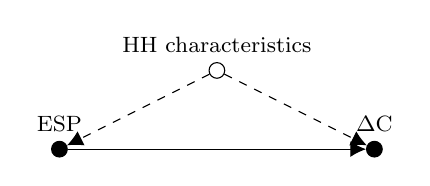
\begin{tikzpicture}[scale=1,font=\footnotesize]
\tikzstyle{s}=[circle,draw,inner sep=2,fill=black]
\tikzstyle{h}=[circle,draw, inner sep=2]
    
    \node[s, label=ESP] (2) at (2,0){};
    \node[s, label=$\Delta$C] (3) at (6,0){};
    \node[h, label=HH characteristics] (4) at (4,1){};
    
    \draw[->] (2) edge (3);
    \draw[->][dashed] (4) edge (2);
    \draw[->][dashed] (4) edge (3);
    
\end{tikzpicture}
\end{frame}

\end{document}